To set up the game, assign one player as the banker; the banker manages the bank's money, houses, hotels, title deed cards, and auctions. The banker may also be a player. The banker gives each player a starting wealth of \rotatebox[origin=c]{180}{\textwon} 1500 (5 x \rotatebox[origin=c]{180}{\textwon} 1, 5 x \rotatebox[origin=c]{180}{\textwon} 5, 4 x \rotatebox[origin=c]{180}{\textwon} 10, 4 x \rotatebox[origin=c]{180}{\textwon} 20, 3 x \rotatebox[origin=c]{180}{\textwon} 50, 2 x \rotatebox[origin=c]{180}{\textwon} 100, 2 x \rotatebox[origin=c]{180}{\textwon} 500 ). Each player chooses a token to move around the board. Additionally, shuffle the community chest and chance cards. To begin the game, place each player’s token on the GO space. On each turn, a player rolls two fair dice, then moves the sum. Figure 1 shows the board layout \citep{gameboard_photo}. The board has 40 landable spaces. Game movement is circular, so once a player reaches the 40th landable space, movement resumes on the 1st landable space. The action taken after moving the token by the sum of the dice depends on the type of space landed on.

\begin{figure}[h]
\centering
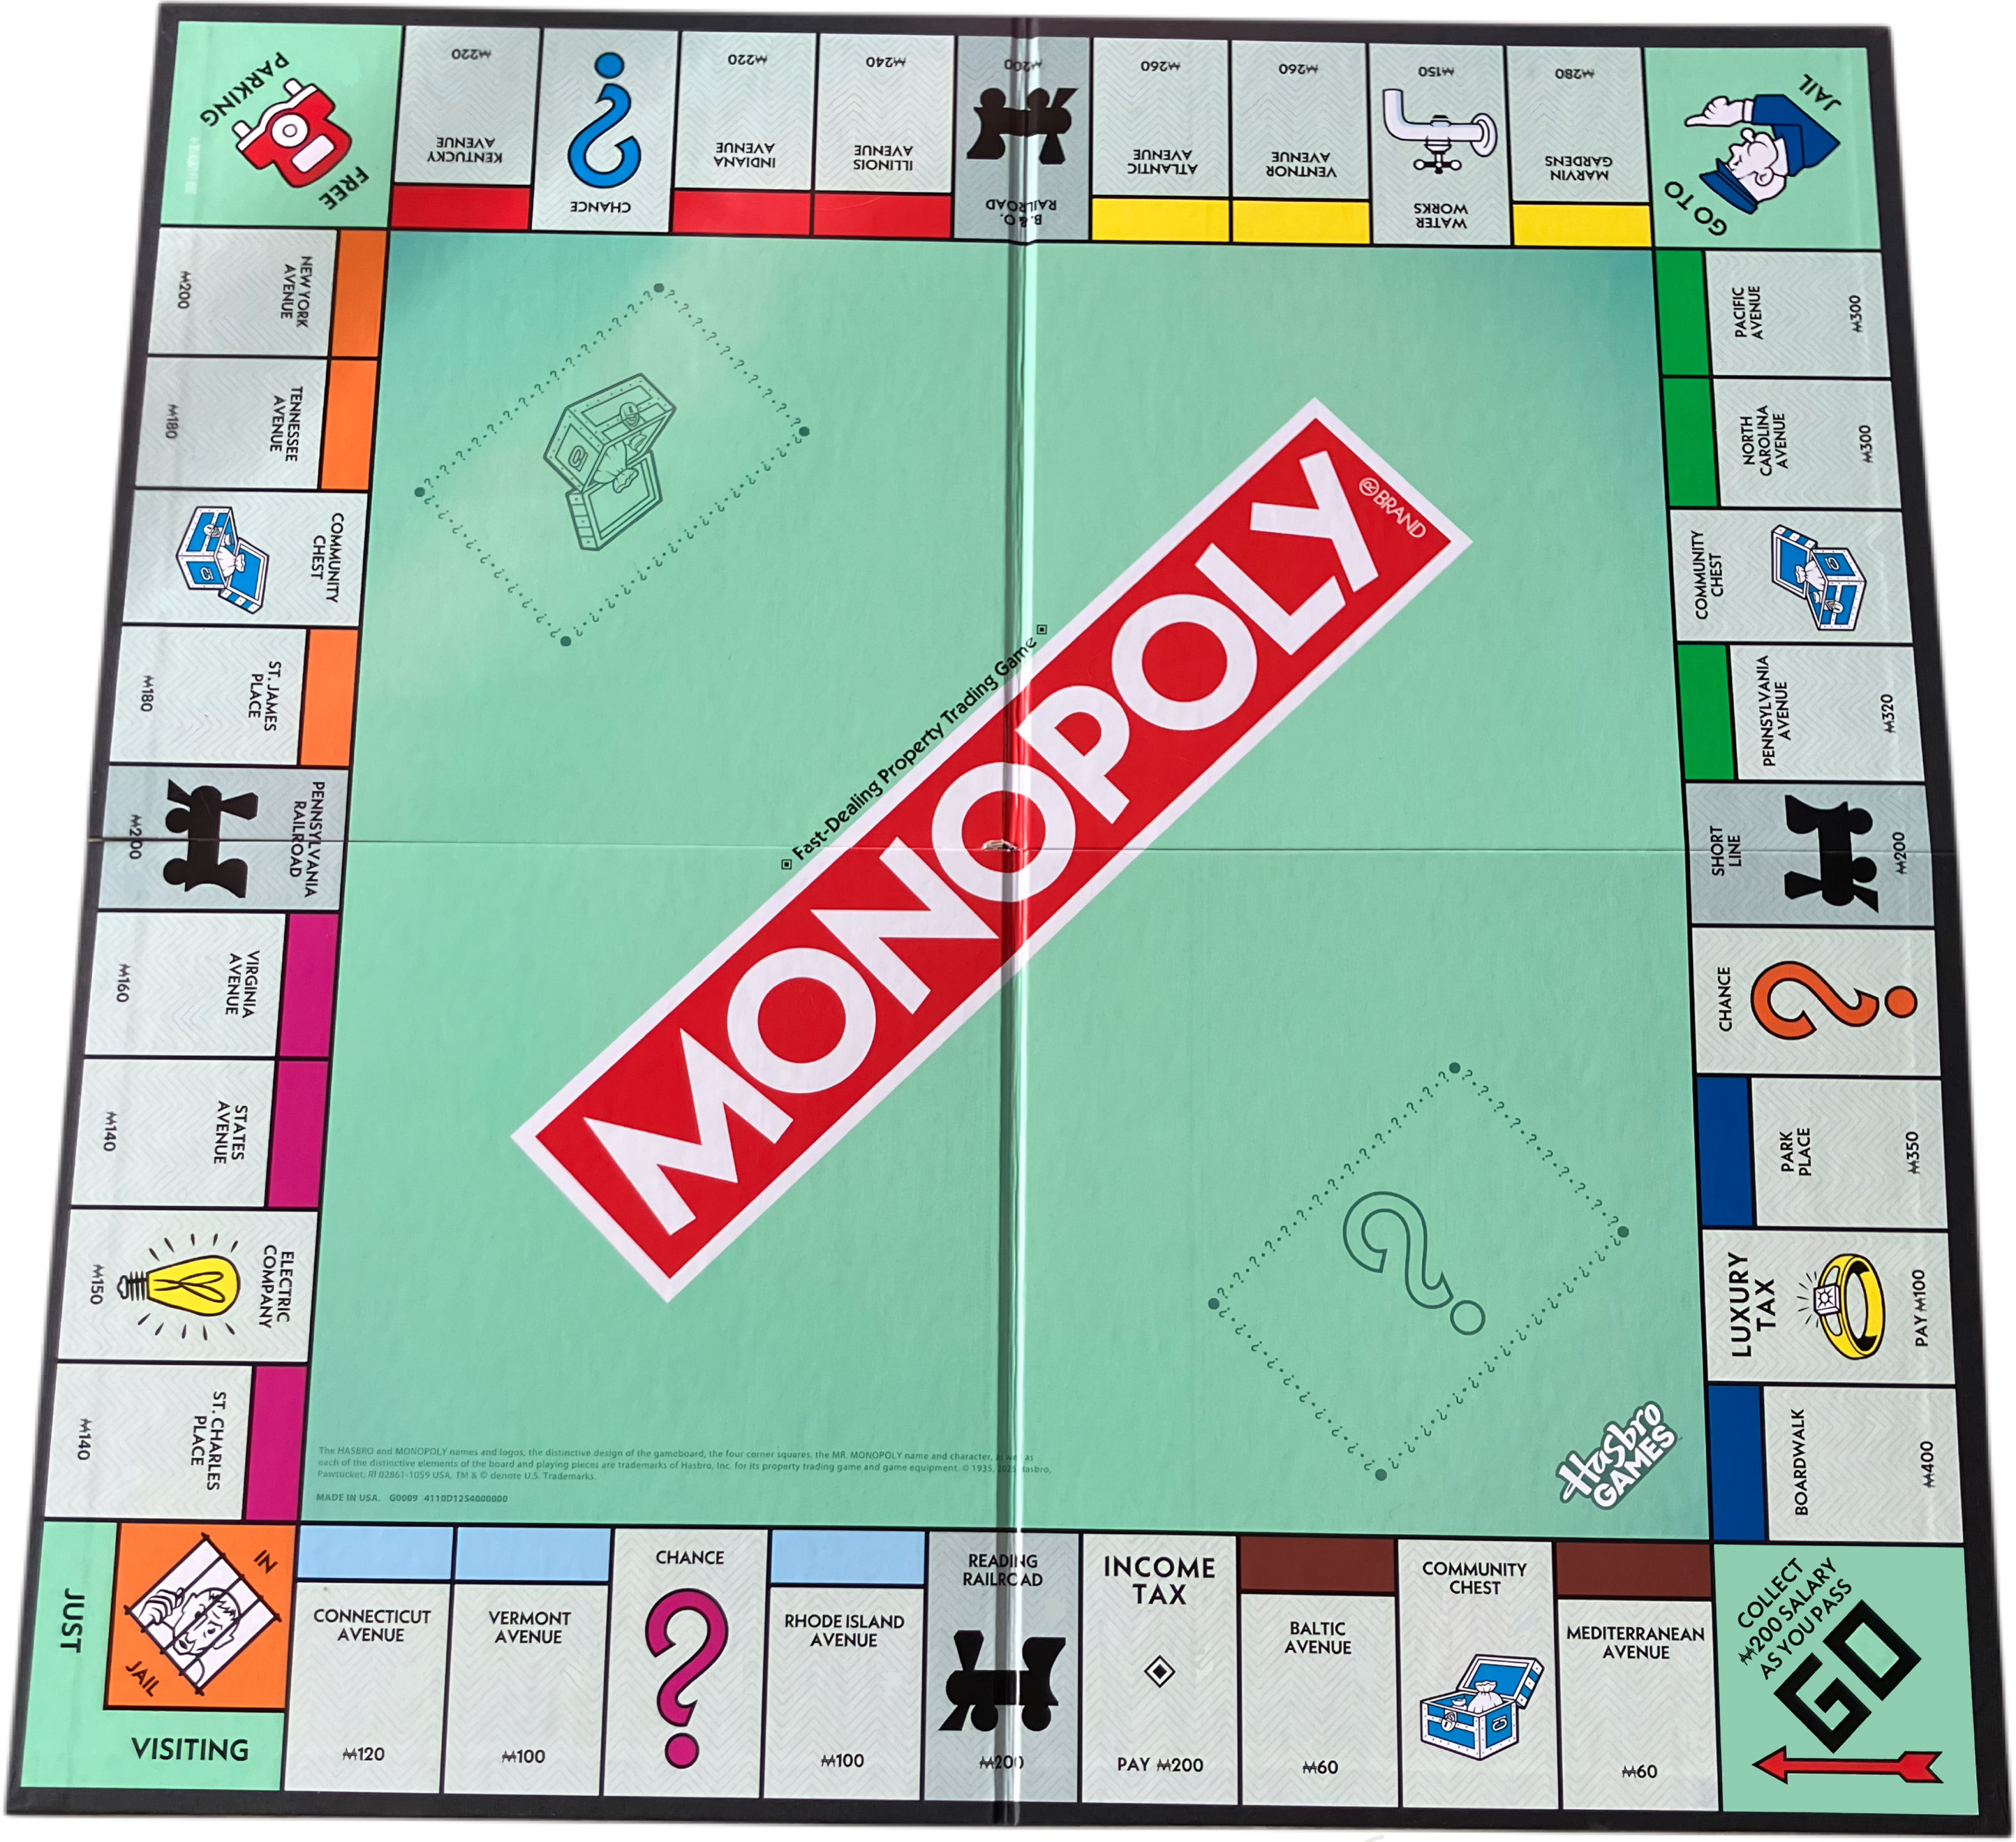
\includegraphics[width=10cm]{figures/gameboard}
\caption{Monopoly GameBoard \citep{gameboard_photo}.}
\label{board}
\end{figure}